%!TEX root = ../thirdYearReport.tex
\appendix
\section{List of dissemination events}
%%%%%%%%%%%%%
%%%%%IIT%%%%%
%%%%%%%%%%%%%

\subsection{IIT contributions to dissemination}

\subsubsection{Invited talks}

\begin{enumerate}
\item  Event: invited researcher at Tokyo University (Japan), Laboratory for Intelligent Systems and Informatics, Department of Mechano-Informatics, School of Information Science and Technology. Period: from October 1, 2015 to October 31, 2015.
\item  Event: invited researcher at AIST (Japan), CNRS-AIST Joint Robotics Laboratory UMI3218/RL (JRL) situated at the Intelligent Systems Research Institute (IS), National Institute of Advance Industrial Science and Technology (AIST). Period: from November 15, 2015 to December 6, 2015.
\end{enumerate}

\subsubsection{International events organisation}

\begin{enumerate}

\item The iCub Summer School, "Veni Vidi Vici", serves to consolidate and disseminate skills in software engineering for humanoid robots. Our goal is to foster collaboration on robot software across the boundaries and lifetimes of specific platforms and projects.
The school focuses on humanoid robotics and will host at least two iCub and a COMAN robot. Students will receive an initial training on the software infrastructure (middleware and tools) and will be required to work on a project of their choice. All participants are expected to be competent C/C++ programmers with an interest in working with others (and an agenda of their own). Info: \url{http://wiki.icub.org/wiki/VVV15}

\begin{figure}[!t]
	\begin{center}
		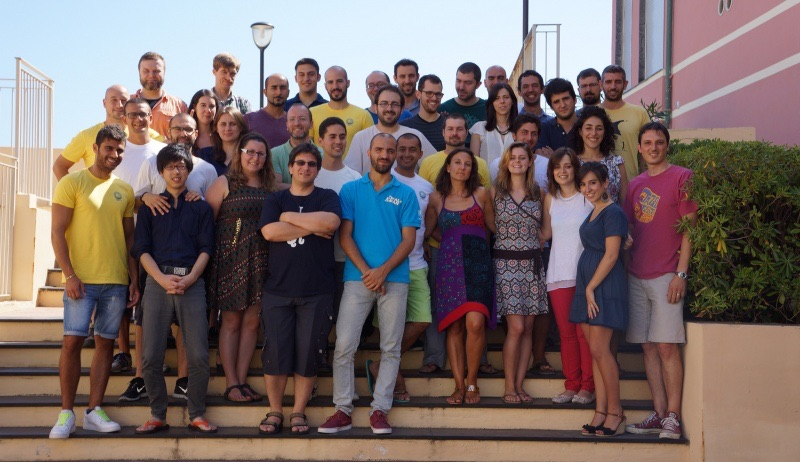
\includegraphics[height=4.5cm]{images/vvv.jpg}
		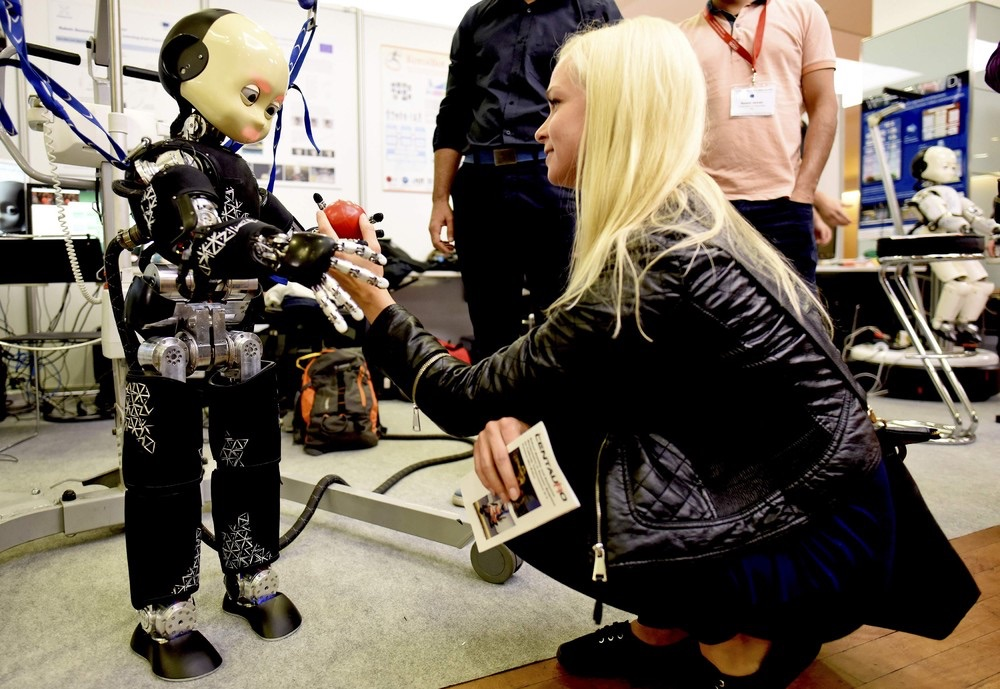
\includegraphics[height=4.5cm]{images/iros.jpg}
		\caption{Left: the iCub Veni-Vidi-Vici summer school. Right: the iCub at the IROS 2015 event organised by the robotics unit at the European Commission.}
		\label{fig:vvv}
	\end{center}
\end{figure}

\item During the IROS 2015 International Conference at Hamburg, different versions of iCub (the Genova Black, and the Heidelberg version) were shown in an exhibition. For three days, iCub interact with visiting people performing different demos, such as torque balancing and the red ball demo. Photo by Fabian Bimmer/Reuters)


\item iCub has been a special guest in Ballar\'o, an italian political show on the public television network.

\item In May, Francesco Nori was an invited speaker at the Creative Mornings event. The talk gave historical and philosophical motivations that guided recent research activities towards the problem of studying how humans interact with the environment and among themselves. The iCub was also presented, as an open-source platform capable of advancing the state-of-the-art in various directions, e.g. decisional autonomy, dependability/adaptability, perception and, in a single all-embracing word, cognitive abilities.

\item In July, during the RSS conference in Rome, a full day workshop titled ``Towards a Unifying Framework for Whole-body and Manipulation Control'' has been organised. Topics covered the following areas:
\begin{itemize}
\item Contacts planning and control
\item Whole-body task control
\item Compliant whole-body movements
\item Dynamics in humanoid robots
\item Machine learning and optimization methods for contact planning and control
\end{itemize}

\item From 22nd of October to 1st of November 2015, the iCub will be showed at the ``Festival della Scienza''. Festival della Scienza, now at its 13th edition, is a publicly opened event which focus on science. During this festival, temporary laboratories and exhibition booths are prepared where researchers and scientists can show and explain to people their work. Presentations are targeted to different audiences, from children to university students to adults. This year festival theme is ``Equilibrium'', and iCub will perform daily showing balancing demos. 

\item Live video shooting at ``Italians got talent'', italian national television show. Shooting: December 1st-3rd 2015. Location: Catanzaro, Italy. The iCub performed the CoDyCo demo based on whole-body torque controlled motions with switching motions.

\item Live demonstrations at the event: ``Italian Manufacturing Forum'', UIC Gleacher Center, Chicago, IL, March 30th, 2016. The iCub was shipped to Chicago to perform several iCub related demonstrations (e.g. iCub standing, iCub performing whole-body equilibrium tasks) at the Italian Manufacturing Forum. 


\end{enumerate}

\subsubsection{Talks at international conferences}

\begin{enumerate}
\item Event: invited talk at the dissemination event Creative mornings. Talk: Interacting with Humans with iCub-humanoid. Dates: Location: May 22nd 2015. Milano, Italy.
\item  Event: Convegno NanoItaly, Roma, 21-24 settembre 2015. Talk: Force and motion capture system
based on distributed micro-accelerometers, gyros, force and tactile sensing. Date: 21 settembre 2015.
\item  Event: International Conference on Humanoid Robotics, 02-06 November 2015. Workshop on Benchmarking bipedal functions of humanoids robots: towards a unified framework. Talk: wholeBodyInterface: a software abstraction layer for benchmarking whole-body motion control. Date: November 3rd 2015.
\item  Event: International Conference on Humanoid Robotics, 02-06 November 2015. Workshop on Reusable and Open-Source Modules for Humanoid Robots. Talk: wholeBodyInterface: An Open- Source Software Abstraction Layer for Whole-Body Motion Control. Date: November 3rd 2015.
\item  Event: International Conference on Humanoid Robotics, 02-06 November 2015. Workshop on Whole-Body Multi-Task Multi-Contact Humanoid Control. Talk: iCub whole-body control through force regulation on rigid non-coplanar contacts. Date: November 3rd 2015.
\item  Event: invited researcher at Université Paris Sud (France). University Paris Sud 11, Paris. CIAMS laboratory in the Motor Con- trol and perception team, University Paris-Sud 11, Paris, France. Inviting professors: Prof. Bastien Berret, University Paris-Sud 11 and Prof. Frédéric Jean, ENSTA Paris-Tech, Unité de Math- ématiques Appliquées. Period: from June 1, 2015 to June 30, 2015.
\item  Invited external member and president at Ph.D. defense Université d'Orléans (France). Ph.D. candidate: Adina Panachea. Date: December 10th, 2015.
\end{enumerate}


\subsubsection{Pubblications}

\begin{enumerate}
\item Camoriano R., Traversaro S., Rosasco L., Metta G. \& Nori F. 2016, ‘Incremental Semiparametric Inverse Dynamics Learning’, IEEE International Conference on Robotics and Automation (ICRA), Stockholm, Sweden, May 16-21, 2016.

\item Del Prete A., Mansard N., Ramos O., Stasse O. \& Nori F. 2015, ‘Implementing Torque Control with High-Ratio Gear Boxes and without Joint-Torque Sensors’, International Journal of Humanoid Robotics.

\item Del Prete A., Nori F., Metta G. \& Natale L. 2015, ‘Prioritized Motion-Force Control of Constrained Fully-Actuated Robots: “Task Space Inverse Dynamics”’, Robotics and Autonomous Systems, vol. 63, Part 1, pp. 150–157.

\item Eljaik J., Kuppuswamy N. \& Nori F. 2015, ‘Multimodal sensor fusion for foot state estimation in bipedal robots using the Extended Kalman Filter’, IEEE/RSJ International Conference on Intelligent Robots and Systems (IROS), Hamburg, Germany, October (29 September - 1 October, 2015).

\item Latella C., Kuppuswamy N. \& Nori F. 2015, ‘Force and motion capture system based on distributed micro-accelerometers, gyros, force and tactile sensing’, 2nd International Electronic Conference on Sensors and Applications,.

\item Nori F., Kuppuswamy N. \& Traversaro S. 2015, ‘Simultaneous state and dynamics estimation in articulated structures’, IEEE/RSJ International Conference on Intelligent Robots and Systems (2015), Hamburg, Germany, October (29 September - 1 October, 2015).

\item Nori F., Traversaro S., Eljaik J., Romano F., Del Prete A. \& Pucci D. 2015, ‘iCub whole-body control through force regulation on rigid non-coplanar contacts’, Frontiers in Robotics and AI.

\item Paikan A., Traversaro S., Nori F. \& Natale L. 2015, ‘Generic Testing Framework for Test Driven Development of Robotic Systems’, in Jan Hodicky (ed.),Modelling and Simulation for Autonomous Systems Workshop, Springer International Publishing pp.216-225, , Prague, Czech Republic, 2015.

\item Pucci D., Romano F. \& Nori F. 2015, ‘Collocated Adaptive Control of Underactuated Mechanical Systems’, IEEE Transactions on Robotics.

\item Romano F., Del Prete A., Mansard N. \& Nori F. 2015, ‘Prioritized Optimal Control: a Hierarchical Differential Dynamic Programming approach’, IEEE International Conference on Robotics And Automation, Seattle, Washington, USA.

\item Traversaro S., Del Prete A., Ivaldi S. \& Nori F. 2015, ‘Inertial parameters identification and joint torques estimation with proximal force/torque sensing’, IEEE International Conference on Robotics and Automation, Seattle, USA, May 26th - 30th, 2015.

\item Traversaro S., Pucci D. \& Nori F. 2015, ‘In Situ Calibration of Six-Axis Force-Torque Sensors using Accelerometer Measurements’, IEEE International Conference on Robotics and Automation, pp.6,  Seattle, USA, May 26th - 30th, 2015.
\end{enumerate}
	
\subsubsection{Media coverage}

\begin{itemize}

\item \url{http://video.repubblica.it/edizione/genova/genova-icub-il-robot-bambino-ora-sta-in-piedi/167466/165953}

\item \url{http://www.nextme.it/tecnologia/robotica/8958-icub-robot-morbidi-8-anni-video}

\item \url{http://video2k.is/index.php/videos/v/jaTEbCsFp_M/yt}

\item \url{http://meta-guide.com/videography/100-best-icub-robot-videos/}

\item \url{http://www.33rdsquare.com/2015/02/icub-becomes-master-of-balancing.html}

\item \url{http://video.corriere.it/robot-icub-fa-progressi-equilibrio/a20154ce-c961-11e4-84dd-480351105d62}

\item \url{http://www.geniuslab.org/storie/con-il-raggiungimento-dellequilibrio-icub-accorcia-i-tempi-per-entrare-nelle-nostre-case/}

\item \url{http://www.rainews.it/dl/rainews/media/Occhi-grandi-e-sorrisone-il-cucciolo-robot-muove-i-primi-passi-93898c5e-032b-4f2f-9240-14ee1682e87c.html}

\item \url{https://www.youtube.com/watch?v=jtjBsBE5GIIandt=3m36s}

\item \url{http://www.rai.tv/dl/RaiTV/programmi/media/ContentItem-38aee841-5df8-48e2-ba54-064c0457bc45.html#p=0}
\end{itemize}

\subsubsection{iCub at international events}

\begin{itemize}
\item CISCO conference Milano 26/1/2015
\item Geo \& Geo Roma 25/2/2015
\item Lancio cartone Transformers 1/3/2015
\item ERF Vienna, workshop on humanoids in the laboratory (chimica, ecc.) 12/3/2015
\item Conferenza stampa De Agostini (lancio X-makers) Barcellona 26/3/2015
\item ITURO conference Istanbul, keynote 11/4/2015
\item CSIFT Shanghai, investors presentation 22-24/4/2015
\item Bal Robotov, invited forum on robotics, Mosca 29/4/2015
\item Robobusiness, invited, Milan 30/4/2015
\item Summer school on Sensing, Lille 21/5/2015
\item Boston Woodshole, summer school CBMM, Robotics Afternoon, 18-22/8/2015
\item Sky International, TV, 25/8/2015
\item Uno Mattina, Rai1, 1/9/2015
\item Rai Petrolio, 10/9/2015
\item Expo, Padiglione Italia, 15/9/2015
\item Aimeta conference, keynote, Genova, 16/9/2015
\item Researchers night, invited, L’Aquila 26/9/2015
\item Trieste Next Fest, invited, Trieste 27/9/2015
\item IROS, Hamburg 28/9, 2/10/2015
\item Caidate scientific talks, Caidate, 3/10/2015
\item Space Challenge, keynote/lecture, Sofia, 6/10/2015
\item Italian Manufacturing Forum, Chicago, IL, 30/03/2016
\end{itemize}

%%%%%%%%%%%%%
%%%%TUD%%%%%%
%%%%%%%%%%%%%
\subsection{TUD contributions to dissemination}

9 invited talks, 1 organised international events, 12 publications (2 journal articles, 10 international conferences), 3 media coverage events, 3 M.Sc. theses and one Ph.D. thesis. 

\subsubsection{Invited talks}

\begin{enumerate}
%year three (03.2015-02.2016)

% Roberto
\item Talk by Roberto Calandra, 16 Oct 2015 University College London, London, UK, host: Guy Lever.
\item Talk by Roberto Calandra, 14 Oct 2015 University of Oxford, Oxford, UK, host: Michael Osborne, Machine Learning Research Group.
\item Talk by Roberto Calandra, 13 Oct 2015 Imperial College London, London, UK, host: Stefan Leutenegger, Dyson Robotics Lab.
\item Talk by Roberto Calandra, 03 Jun 2015 University of British Columbia, Vancouver, Canada, host: Mark Schmidt.
\item Talk by Roberto Calandra, 02 Jun 2015 University of Washington, Seattle, US, host: Dieter Fox, Robotics and State Estimation Lab.
\item Talk by Roberto Calandra, 01 Apr 2015 TU Freiburg, Freiburg, Germany, host: Frank Hutter.

%Elmar
\item Talk by Elmar Rueckert, 11/2015 Understanding Human Motor Control through Robotics Applications. Invited Talk in Prof. Constantin Rothkopf’s seminar on ’research and applications of psychology in IT’, Darmstadt, Germany.
\item Talk by Elmar Rueckert, 02/2015 Probabilistic Inference and Modeling of Human Motor Skill Learning. Invited Talk. Workshop with Marc Toussaint’s group, Wolfram Burgard’s group and Oliver Brock’s group, Manigod, France.


%Jan
\item Talk by Jan Peters, 06/2015 Universit\"at Ulm, Host: F.~Kargl, Ulm, Germany, July, 2015.
% \item Talk by Jan Peters, 9/17/2014 IEEE/RSJ International Conference on Intelligent Robots and Systems (IROS), Session [1] Keynote for the Learning by Demonstration Session Topic, Chicago, USA
% \item Talk by Jan Peters, 7/16/2014 13th International Conference on Intelligent Autonomous Systems (IAS-13), Padua, Italy 
% \item Talk by Jan Peters, 7/11/2014 British Machine Vision Association (Vision for language and manipulation), London, UK
% \item Talk by Jan Peters, 7/9/2014 IEEE/ASME Conference on Advanced Intelligent Mechatronics (AIM2014), Besancon, France
% \item Talk by Jan Peters, 3/27/2015 RSS 2015 Symposium: Frontiers of Robotics, New Brunswick, USA 
% \item Talk by Jan Peters, 9/14/2014 IROS Workshop: Machine Learning in Planning and Control of Robot Motion, Chicago, USA
% \item Talk by Jan Peters, 6/5/2014 ICRA Workshop: iCub and Friends, Hong Kong, China
% \item Talk by Jan Peters, 2/6/2015 Carnegie Mellon University, Robotics Institute Lecture Series , Host: S. Srinivasa, J.A. [55] Bagnell, Pittsburgh, PA, USA
% \item Talk by Jan Peters, 1/16/2015 Technische Universität München, Host: E. Steinbach, Munich, Germany [56]
% \item Talk by Jan Peters, 12/4/2014	KIT, Host: W. Juling, Karlsruhe, Germany [57]
% \item Talk by Jan Peters, 11/28/2014	ETH Zürich, ETH Distinguished Lecture Series, Host: R. Siegwardt, Zürich, Switzerland
% \item Talk by Jan Peters, 7/7/2014 Universität Hamburg, Host: U. von Luxburg, Hamburg, Germany [59]
% \item Talk by Jan Peters, 5/9/2014 Université de Liege, Host: D. Ernst, Liege, Belgium [60]
% \item Talk by Jan Peters, 2/5/2014 ABB AG, Corporate Research Center, Robotics and Manufacturing, Host: H. Ding, Ladenburg, Germany
% \item Talk by Jan Peters, 2/4/2014 Technical University of Graz, Host: W. Maas, Graz,Austria [62]
\end{enumerate}


\subsubsection{Publications}

\begin{enumerate}
%year three (03.2015-02.2016)
%journals
\item E Rueckert, D Kappel, D Tanneberg, D Pecevski and J Peters. Recurrent Spiking Networks Solve Planning Tasks. Scientific Reports, Nature Publishing Group, 2016.
\item R Calandra, A Seyfarth, J Peters and M P Deisenroth. Bayesian optimization for learning gaits under uncertainty. Annals of Mathematics and Artificial Intelligence, pages 1–19, 2015.
%conferences
\item J Kohlschuetter, J Peters and E Rueckert. Learning Probabilistic Features from EMG Data for Predicting Knee Abnormalities. In Proceedings of the XIV Mediterranean Conference on Medical and Biological Engineering and Computing (MEDICON), 2016.
\item V Modugno, G Neumann, E Rueckert, G Oriolo, J Peters and S Ivaldi. Learning soft task priorities for control of redundant robots. In Proceedings of the International Conference on Robotics and Automation (ICRA), 2016.
\item R Calandra, S Ivaldi, M Deisenroth, E Rueckert and J Peters. Learning Inverse Dynamics Models with Contacts. In Proceedings of the International Conference on Robotics and Automation (ICRA). 2015.
\item R. Calandra, S. Ivaldi, Marc. P. Deisenroth, E. Rueckert, and J. Peters. Learning inverse dynamics models with contacts using tactile sensors. ICRA 2015 Workshop on Tactile \& force sensing for autonomous, compliant, intelligent robots, 2015.
\item E Rueckert, J Mundo, A Paraschos, J Peters and G Neumann. Extracting Low-Dimensional Control Variables for Movement Primitives. In Proceedings of the International Conference on Robotics and Automation (ICRA). 2015. 
\item S Traversaro, A Del Prete, S Ivaldi and F Nori. Avoiding to rely on Inertial Parameters in Estimating Joint Torques with proximal F/T sensing. In Proceedings of the International Conference on Robotics and Automation (ICRA). 2015.
\item A Paraschos, E Rueckert, J Peters and G Neumann. Model-free Probabilistic Movement Primitives for physical interaction. In Intelligent Robots and Systems (IROS), 2015 IEEE/RSJ International Conference on. 2015, 2860–2866. 
\item E Rueckert, R Lioutikov, R Calandra, M Schmidt, P Beckerle and J Peters. Low-cost Sensor Glove with Force Feedback for Learning from Demonstrations using Probabilistic Trajectory Representations. In ICRA 2015 Workshop on Tactile and force sensing for autonomous compliant intelligent robots. 2015.
\item L Fritsche, F Unverzag, J Peters and R Calandra. First-person tele-operation of a humanoid robot. In Humanoid Robots (Humanoids), 2015 IEEE-RAS 15th International Conference on. 2015, 997–1002.
\item R Calandra, S Ivaldi, M P Deisenroth and J Peters. Learning torque control in presence of contacts using tactile sensing from robot skin. In Humanoid Robots (Humanoids), 2015 IEEE-RAS 15th International Conference on. 2015, 690–695.
\end{enumerate}

\subsubsection{Media coverage}%year three (03.2015-02.2016)

\begin{enumerate}
%Elmar
\item 09/2015 Organized by Elmar Rueckert, Kinderuni Darmstadt. Interactive robot demonstrations of the Nao, the ICub and the Darias robots. Supported by Veronika Weber and Guilherme J. Maeda.
\item 04/2015 Interview of Jan Peters, Major German TV program, SAT1. Life demonstrations of teaching the ICub how to stack cup.
\item 03/2015 Organized by Elmar Rueckert, KID Science Radioclub. Lab tour and life demonstrations of the Oncilla, the ICub and the Darias robots. Supported by Veronika Weber, Guilherme J. Maeda, Rudolf Lioutikov and Roberto Calandra.

%Jan, list below is from year two
% \item http://www.1730live.de/intelligente-maschinen/
% \item 2/17/2015 Focus, Müssen wir uns bald vor intelligenten Systemen fürchten?, Germany
% \item 10/21/2014 Wired (German Edition), Aus Fails lernen: Roboter der TU-Darmstadt optimieren sich autonom,
% \item 2/12/2015 Frankfurter Rundschau, Menschliche Maschinen, Germany, by Franziska Schubert. 
% \item 12/1/2014 Hoch3, Ich kann täglich mehr, Germany.
% \item 9/17/2014 The Guardian, Win tickets to see what tomorrow?s world may hold, UK.
% \item 28/3/2014 DRadio Wissen, Tischtennisroboter: Falscher Aufschlag, Germany.
\end{enumerate}

\subsubsection{MSc. and Ph.D. theses}%year three (03.2015-02.2016)
\begin{enumerate}
 \item Stark S. MSc. thesis. Learning Probabilistic Feedforward and Feedback Policies for Generating Stable Walking Behaviors. 2016.
 \item Kohlschuetter J. MSc. thesis. Learning Probabilistic Classifiers from Electromyography Data for Predicting Knee Abnormalities. 2016.
 \item D Tanneberg. MSc. thesis. Spiking Neural Networks Solve Robot Planning Problems. 2016.
 \item O Kroemer. Machine Learning for Robot Grasping and Manipulation. 2015.
\end{enumerate}

\subsubsection{Student research stays}

\begin{enumerate}
 \item E Rueckert, 2014. Jozef Stefan Institute, Slovenia, Department of Automation, Biocybernetics and Robotics, Prof. Dr. Jan Babic. Research internship on investigating the functional role of supportive contacts in human postural control. 
\end{enumerate}

\subsubsection{Organised conference workshops}

\begin{enumerate}
\item  R.~Calandra: Organizer of the Workshop on Bayesian Optimization (BayesOpt) at NIPS 2015. Web: http://bayesopt.github.io/
\end{enumerate}

%here is our list from the last year
% \begin{enumerate}
% \item  ICRA 2015: organizer of Workshop "Tactile and force sensing for autonomous, compliant and intelligent robots?. Web: http://www.ausy.tu-darmstadt.de/Workshops/ICRA2015TactileForce 
% \end{enumerate}

%\subsubsection{Meetings with industrial partners}

%TACMAN List
%\begin{enumerate}
%*** TUDA
%\item  H.~van Hoof, ``Research visit'', \emph{SynTouch}, Los Angeles, USA, May, 2015.
%\item  F.~Veiga, ``Research visit'', \emph{DLR}, Oberpfaffenhofen, Germany, December, 2015.
%\end{enumerate}

\subsubsection{Invited speakers}%year three (03.2015-02.2016)
\begin{enumerate}
	\item W.~Kellermann, Invited Speaker at TUDA, \emph{Friedrich-Alexander Univerisit\"at Erlangen-N\"urnberg}, Erlangen, Germany, December, 2015.
	\item D.~Nikolic, Invited Speaker at TUDA, \emph{Max-Planck Institut for Brain Research}, Frankfurt, Germany, January, 2016.
	\item V.~Lippi, Invited Speaker at TUDA, \emph{Uniklinik Freiburg}, Freiburg, Germany, February, 2016.
	\item F.~Hutter, Invited Speaker at TUDA, \emph{Universit\"at Freiburg}, Freiburg, Germany, February, 2016.
\end{enumerate}

\subsubsection{Collaborations}

%ACTIVE collaborations where TUD is involved.
\begin{enumerate}%Note: names are listed in alphabetical order
	\item UB and TUD, involved are M.~Azad, M.~Mistry, J.~Peters, E.~Rueckert. Title: \emph{Uncertainty in contact}, first results on TUD's ICub. Paper submission planned for a robotics conference (HUMANOIDS, ICRA) in 2016. 
	\item TUD and JSI, involved are J.~Babic, J.~Camernik, J.~Peters, E.~Rueckert. Title: \emph{Postural control predicts volitional motor control}, paper submitted for review at Scientific Reports, 01/2016.
\end{enumerate}
%Planned collaborations are not listed. Here is a list:
%IIT, UB, TUD: D.~Pucci and E.~Rueckert discussed at IIT in Nov.2015 a potential collaboration on comparing balancing controller on the ICub. Based on the collaboration between UB and TUD
%JSI, TUD: J.~Babic and E.~Rueckert discussed in January, 2016 a follow-up collaboration on Probabilistic models of human motion.  
%UPMC and TUD, involved are R.~Lober, G.~Neumann, V.~Padois, A.~Paraschos, J.~Peters, E.~Rueckert., O.~Sigaud. 

%%%%%%%%%%%%%
%%%%UPMC%%%%%
%%%%%%%%%%%%%
\subsection{UPMC contributions to dissemination}

3 invited talks, 0 organised international events, 6 publications (6 internal conferences), 1 media coverage events

\subsubsection{Invited talks}

\begin{enumerate}
\item Aurélien Ibanez, Vincent Padois, Philippe Bidaud - "Whole-body control of humanoid robots and virtual humans at ISIR: Multi-objective activities, locomotion and Model Predictive Control" - Invited talk at the French-German-Japanese Conference on Humanoid and Legged Robotics (HLR) - Heidelberg,  Germany - May 2014.

\item Olivier Sigaud - "Towards robots immersed in our society: where are we now?" - Invited talk at  the cognitive science student society of Marseille" -  Marseille, France - March 2015.

\item Vincent Padois - ?Issues and challenges of interactive robotics in complex industrial contexts". Invited talk at the Cap Digital/Innorobo day about ?Robotics et Innovations?, Lyon, France - March 2014.
\end{enumerate}

\subsubsection{Publications}
R Lober, V Padois and O Sigaud. Multiple Task Optimization using Dynamical Movement Primitives for Whole-Body Reactive Control. In Proceedings of the IEEE-RAS International Conference on Humanoid Robots (Humanoids). 2014

M Liu, S Hak and V Padois. Generalized Projector for Task Priority Transitions During Hierarchical Control. In Proceedings of the IEEE International Conference on Robotics and Automation. 2015.

S Ivaldi, J Peters, V Padois and F Nori. Tools for simulating humanoid robot dynamics: a survey based on user feedback. In Proceedings of the IEEE-RAS International Conference on Humanoid Robots (Humanoids). November 2014.

Aurélien Ibanez, Philippe Bidaud and Vincent Padois. Automatic optimal biped walking as a Mixed-Integer Quadratic Program. In J Lenar\v ci\v c and O Khatib (eds.). Advances in Robot Kinematics. Springer International Publishing, 2014, pages 505-516. DOI BibTeX

Aurélien Ibanez, Philippe Bidaud and Vincent Padois. Emergence of humanoid walking behaviors from Mixed-Integer Model Predictive Control. In Proceedings of the IEEE/RSJ International Conference on Intelligent Robots and Systems. 2014. DOI BibTeX

Aurélien Ibanez, Philippe Bidaud and Vincent Padois. A Distributed Model Predictive Control approach for robust postural stability of a humanoid robot. In Proceedings of the IEEE International Conference on Robotics and Automation. June 2014. BibTeX

Aurélien Ibanez, Philippe Bidaud and Vincent Padois. Automatic optimal biped walking as a Mixed-Integer Quadratic Program. In Proceedings of the 14th International Symposium on Advances in Robot Kinematics. July 2014. BibTeX

\subsubsection{Media coverage}

Olivier Sigaud - "Robolution" - Documentary by  V. Gonon and X. Sayanoff for the "Cine + Frisson" - December 2014.

%%%%%%%%%%%
%%%%UB%%%%%
%%%%%%%%%%%
\subsection{UB contributions to dissemination}

3 invited talks, 0 organised international events, 5 publications (5 internal conferences), 0 media coverage events

\subsubsection{Invited talks}

\begin{enumerate}
\item Invited Talk at Human Motion Modeling and Human Inspired Motor Control Workshop, Humanoids 2014
\item Invited Lecturer at European Computational Motor Control Summer School, 6/2014
\item Invited Talk at Honda Research Europe, 6/2014
\end{enumerate}

\subsubsection{Publications}

M Azad, M Mistry, Balance Control Strategy for a Robot with Compliant Contacts, Int. Conf on Robotics and Automation, 2015.

NT Alberto, M Mistry, F Stulp, Computed Torque Control with Variable Gains through Gaussian Process Regression, Int. Conf. on Humanoid Robotics, 2014.

M Azad, J Babic, M Mistry, Effects of Hand Contact on the Stability of a Planar Humanoid with a Momentum Based Controller, Int. Conf. on Humanoid Robotics, 2014.

V Ortenzi, M Adjigble, K Jeffery, R Stolkin, M Mistry, An experimental study of robot control during environmental contacts based on projected operational space dynamics, Int. Conf. on Humanoid Robotics, 2014.

M. Azad and R. Featherstone, Balancing control algorithm for a 3D under-actuated robot, Proceedings of the IEEE/RSJ International Conference on Intelligent Robots and Systems, Chicago, Illinois, 14-18 September 2014.

%%%%%%%%%%%%%
%%%%JSI%%%%%%
%%%%%%%%%%%%%
\subsection{JSI contributions to dissemination}

2 invited talks, 1 editorial for journal special issue, 3 publications (2 journal, 1 internal conferences), 0 media coverage events.

\subsubsection{Invited talks}

\begin{enumerate}

\item Babic, Jan. Human-in-the-loop control of robots for industrial assembly tasks : invited talk, Omron Keihanna Technology Innovation Center, 7th September 2015, Kyoto, Japan.

\item Babic, Jan. Compliant robotic behaviour through human sensorimotor adaptation : presented at ICRA 2015, IEEE International Conference on Robotics and Automation, May 26th-30th, 2015, Seattle, Washington, USA.

\end{enumerate}

\subsubsection{Editorial work}

\begin{enumerate}
	
\item Babic, J. Guest editor of Autonomous robots, Kluwer Academic Publishers, 1994-. ISSN 0929-5593. http://link.springer.com/journal/10514.

\end{enumerate}

\subsubsection{Publications}

Ivaldi, S., Babic, J., Mistry, M., Murphy, R. Special issue on whole-body control of contacts and dynamics for humanoid robots. Autonomous robots, 2016, vol. 40, no. 3, 425-428.
 
Peternel, L., Noda, T., Petric, T., Ude, A,. Morimoto, J., Babic, J. Adaptive control of exoskeleton robots for periodic assistive behaviours based on EMG feedback minimisation. PloS one, ISSN 1932-6203, 2016, vol. 11, no. 2, 0148942-1-0148942-26.

Peternel, L., Petric, T., Babic, J. Human-in-the-loop approach for teaching robot assembly tasks using impedance control interface. In: 2015 IEEE International Conference on Robotics and Automation, May 26th-30th, 2015, Seattle, Washington, USA. ICRA 2015. Danvers: IEEE = Institute of Electrical and Electronics Engineers, cop. 2015, 1497-1502.

%%%%%%%%%%%%%
%%%%INRIA%%%%
%%%%%%%%%%%%%
\subsection{INRIA contributions to dissemination}

4 invited talks, 4 organised international events, 8 publications (4 journal, 4 internal conferences), 3 media coverage events

\subsubsection{Invited talks}
\begin{enumerate}
\item Ivaldi, S. (2014) iCub interacting with humans: software tools and best practices. Invited talk at IEEE Humanoids 2014 Workshop - One day with a humanoid robot.
\item Ivaldi, S. (2014) Social learning and engagement in human-humanoid interactions. Invited talk at IAS13 Workshop on Evaluating social robots.
\item  Ivaldi, S. (2014) Humanoids and dynamics estimation and simulation. Invited talk at French-German-Japan Workshop on Humanoid and Legged robots.
\item Ivaldi, S. (2014) iCub learning from humans via multimodal, physical, social and natural interaction: experiments from MACSi, EDHHI and CODYCO projects. Invited talk at IEEE ICRA 2014 Workshop - iCub and friends.
\end{enumerate}


\subsubsection{Organised workshop/special sessions}
\begin{enumerate}
\item  ICRA 2015: organizer of Workshop "Tactile and force sensing for autonomous, compliant and intelligent robots?. Web: http://www.ausy.tu-darmstadt.de/Workshops/ICRA2015TactileForce 
\item  ICRA 2015: member of the Program Committee of the Workshop "Compliant and Versatile Robot Control in Human Environments: Bridging the Gap between Learning and Control?. Web: http://cs.stanford.edu/people/khansari/ICRA2015/index.html 
\item  2014: Preliminary results of project EDHHI: where do people gaze and touch during HRI?
Invited talk at Journée LABEX SeNSE by Catherine Achard
\item  2014: Robot learning through interaction with humans
Invited talk at Telecom-ParisTech by Catherine Pelachaud
\end{enumerate}


\subsubsection{Media coverage}
\begin{enumerate}
\item  March 2015, interview at Radio 24 in the program ?Giovani Talenti?:
http://www2.radio24.ilsole24ore.com/blog/nava/2015/03/14/ricercatrice-di-robotica-in-francia/
\item  September 2014, article on ?Le point? (french newspaper)
\url{http://www.lepoint.fr/villes/l-appartement-de-demain-15-09-2014-1863287_27.php}
\item  April 2014, article and comics on the blog L?Avventura on The Monde (french national newspaper) \url{http://lavventura.blog.lemonde.fr/2014/04/07/qui-a-peur-du-robot-google/}
\end{enumerate}

\subsubsection{Publications}
Anzalone, S.; Boucenna, S.; Ivaldi, S.; Chetouani, M. (2015) Evaluating the engagement with social robots. International Journal of Social Robotics. In press.

Droniou, A.; Ivaldi, S.; Sigaud, O.  (2014) Deep unsupervised network for multimodal perception, representation and classification. Robotics and Autonomous Systems.

Saut, J.-P.; Ivaldi, S.; Sahbani, A.; Bidaud, P.  (2014) Grasping objects localized from uncertain point cloud data. Robotics and Autonomous Systems, vol 62, n. 12, pp.1742?1754.

Ivaldi, S.; Anzalone, S.M.; Rousseau, W.; Sigaud, O.; Chetouani, M. (2014) Robot initiative in team learning task increases the rhythm of interaction but not the perceived engagement. Frontiers in Neurorobotics. Vol 8, No 5, DOI 10.3389/fnbot.2014.00005.

Calandra, R.; Ivaldi, S.; Deisenroth, M.P.; Rueckert, E.; Peters, J. (2015). Learning Inverse Dynamics Models with Contacts, Proc. IEEE International Conference on Robotics and Automation (ICRA). 

Traversaro, S.; Del Prete, A.; Ivaldi, S.; Nori, F. (2015). Avoiding to rely on Inertial Parameters in Estimating Joint Torques with proximal F/T sensing, Proc. IEEE International Conference on Robotics and Automation (ICRA). 

Ivaldi, S.; Peters, J.; Padois, V.; Nori, F. (2014). Tools for simulating humanoid robot dynamics: a survey based on user feedback, Proceedings of the International Conference on Humanoid Robots (HUMANOIDS).

Droniou, A.; Ivaldi, S.; Sigaud, O. (2014). Learning a repertoire of actions with Deep Neural Networks, Proceedings of the Int. Conf. on Development and Learning (ICDL).

Nori, F.;  Peters, J.; Padois, V.; Babic, J.; Mistry, M.; Ivaldi, S.  (2014) Whole-body Motion in Humans and Humanoids. Workshop New Research Frontiers for Intelligent Autonomous Systems ? NRF-IAS-2014. Invited paper.


